%% LyX 2.1.1 created this file.  For more info, see http://www.lyx.org/.
%% Do not edit unless you really know what you are doing.
\documentclass[english]{article}
\usepackage{graphicx}
\usepackage[T1]{fontenc}
\usepackage[latin9]{inputenc}
\usepackage{amstext}
\usepackage{amsmath}
\usepackage{babel}
\usepackage{courier}
\usepackage[margin=1in]{geometry}

\begin{document}

\title{Design Document: \\Matrix Product State for Probability Dynamics}


\author{Peter Gjeltema (gjeltema@princeton.edu)
	   \\ Peiqi Wang (peiqiw@princeton.edu)
	    \\ Jun Xiong (xiong@princeton.edu) 
	    \\ Bin Xu (binx@princeton.edu) 
	    \\ Liangsheng Zhang(liangshe@princeton.edu)}
	    
\date{}

\maketitle

\section{Introduction}

Matrix product state (MPS) is a novel numerical algorithm that is
widely used in quantum many body physics. For a problem of quantum
spin chains, the states live in a Hilbert space expanded by the states
of each spin (refered to as ``orbitals'' hereafter). The dimension
of that Hilbert space is $m^{N}$ where each orbital has $m$ choices
and we get $N$ orbitals in total. As the dimension of state space
grows exponentially with $N$, the simulation can be extremely hard
when dealing with a few dozens of spins. 

In 1995, White (S. R. White, Phys. Rev. Lett. 69, 2863 (1992)) proposed
the density matrix renormalization group blah blah blah, and then
Schollwock (arXiv: 1008.3477, this one describes everything) and then
Vidal and blah blah blah...

\section{Background}

\subsection{The difficult many body problem}

When we have a state as a vector in the Hilbert space, it is expressed
as

\[
|\psi\rangle=\sum_{\{\sigma_{i}\}}A_{\{\sigma_{i}\}}|\sigma_{1}\sigma_{2}\sigma_{3}\cdot\cdot\cdot\sigma_{N}\rangle
\]
where $|\sigma_{1}\sigma_{2}\sigma_{3}\cdot\cdot\cdot\sigma_{N}\rangle$
is a product basis of the local Hilbert space on different sites.

Applying a linear time-evolution operator $\hat{O}$ on this state,
the general form of $\hat{O}$ is

\[
\hat{O}=\sum_{\{\sigma\},\{\sigma'\}}|\sigma'_{1}\sigma'_{2}\sigma'_{3}\cdot\cdot\cdot\sigma'_{N}\rangle\langle\sigma_{1}\sigma_{2}\sigma_{3}\cdot\cdot\cdot\sigma_{N}|O_{\{\sigma'\}\{\sigma\}}\rangle
\]
where $\langle\sigma_{1}\sigma_{2}\sigma_{3}\cdot\cdot\cdot\sigma_{N}|$ is a vector in the dual Hilbert space and $O_{\{\sigma'\}\{\sigma\}}$ is a complex number that represents the amplitude of this map. The application of this operator on the state is naturally written as
\[
\hat{O}|\psi\rangle=\sum_{\{\sigma\},\{\sigma'\}}|\sigma'_{1}\sigma'_{2}\sigma'_{3}\cdot\cdot\cdot\sigma'_{N}\rangle\langle\sigma_{1}\sigma_{2}\sigma_{3}\cdot\cdot\cdot\sigma_{N}|\ O_{\{\sigma'\}\{\sigma\}}\sum_{\{\sigma''_{i}\}}A_{\{\sigma_{''i}\}}|\sigma''_{1}\sigma''_{2}\sigma''_{3}\cdot\cdot\cdot\sigma''_{N}\rangle
\]
Using the orthonomal condition of basis, it can be simplified to

\[
\hat{O}|\psi\rangle=\sum_{\{\sigma_{i}\}\{\sigma'_{i}\}}A_{\{\sigma_{i}\}}O_{\{\sigma'\}\{\sigma\}}|\sigma'_{1}\sigma'_{2}\sigma'_{3}\cdot\cdot\cdot\sigma'_{N}\rangle
\]


Depite its simple form, the actual computation is very difficult since
we need to perform the summation over $N$ indices of $\sigma_{i}$
simutaneously, thus gives $m^{N}$ terms. For the simplest case when
$m=2$ (only two elementary states for one site), $m^{N}\approx10^{9}$
for $N=30$, taking more than $10$ seconds for one single contraction,
which makes the problem intractable.


\subsection{Matrix Product States (MPS)}

To deal with the large number of terms in the contraction, we want
to effectively split the space. Let's focus on the coefficient $A_{\{\sigma_{i}\}}=A_{\sigma_{1}\sigma_{2}\sigma_{3}\cdot\cdot\cdot\sigma_{N}}$.
From a direct point of view, it is a rank-N tensor which has N indices,
but we can group some indices so that it becomes $A_{\sigma_{1}(\sigma_{2}\sigma_{3}\cdot\cdot\cdot\sigma_{N})}$
with only $2$ indices where the first has $m$ possible values and
the second has $m^{N-1}$. Grouping $N-1$ indices means making a
bijection map from $N-1$ numbers varying between $1$ and $m$ to
a single integer varying from $1$ to $m^{N-1}$. This re-indicing
trick is crucial in MPS algorithms.

We can then treat this 2 indices object $A_{\sigma_{1}(\sigma_{2}\sigma_{3}\cdot\cdot\cdot\sigma_{N})}$
as a matrix with $\sigma_{1}$ the row index and $(\sigma_{2}\sigma_{3}\cdot\cdot\cdot\sigma_{N})$
the column index, thus forming a $m\times m^{N-1}$ matrix. Applying
singular value decomposition (SVD) on this matrix gives 
\[
A_{\sigma_{1}(\sigma_{2}\sigma_{3}\cdot\cdot\cdot\sigma_{N})}=U_{m_{1}}^{\sigma_{1}}S_{m_{1}m_{2}}V_{m_{2}(\sigma_{2}\sigma_{3}\cdot\cdot\cdot\sigma_{N})}=U_{m_{1}}^{\sigma_{1}}\tilde{V}_{m_{1}(\sigma_{2}\sigma_{3}\cdot\cdot\cdot\sigma_{N})}
\]
where $U$ is a $m\times m$ unitary matrix and $S$ is a $m\times m$
diagonal matrix with non-negative diagonal elements arranged in decending
order. We can apply a similar procedure on $\tilde{V}_{m_{1}(\sigma_{2}\sigma_{3}\cdot\cdot\cdot\sigma_{N})}$
by re-arranging indices as $\tilde{V}_{m_{1}(\sigma_{2}\sigma_{3}\cdot\cdot\cdot\sigma_{N})}=\tilde{V}_{(m_{1}\sigma_{2})(\sigma_{3}\cdot\cdot\cdot\sigma_{N})}$
and applying a similar SVD:

\[
\tilde{V}_{(m_{1}\sigma_{2})(\sigma_{3}\cdot\cdot\cdot\sigma_{N})}=U_{(m_{1}\sigma_{2})m_{2}}S_{m_{2}m_{2}'}V_{m_{2}'(\sigma_{3}\cdot\cdot\cdot\sigma_{N})}=U_{m_{1}m_{2}}^{\sigma_{2}}\tilde{V}_{m_{2}(\sigma_{3}\cdot\cdot\cdot\sigma_{N})}
\]
where the second ``$=$'' reshapes the $U$ matrix and multiplied
the $S$ and $V$ matrices. 

Noticing that $\tilde{V}_{m_{2}(\sigma_{3}\cdot\cdot\cdot\sigma_{N})}$
is almost the same as $\tilde{V}_{m_{1}(\sigma_{2}\sigma_{3}\cdot\cdot\cdot\sigma_{N})}$
except for having one fewer $\sigma_{i}$, we can apply this precedure
inductively and write the original coefficient tensor as

\[
A_{\{\sigma_{i}\}}=U_{m_{1}}^{\sigma_{1}}U_{m_{1}m_{2}}^{\sigma_{2}}U_{m_{2}m_{3}}^{\sigma_{3}}\cdot\cdot\cdot U_{m_{N-1}m_{N}}^{\sigma_{N}}
\]
This form is called the matrix product state, and $\sigma_{i}$'s
are called ``physical indices'' while $m_{i}$'s are called ``auxiliary
indices''. It worths noting that, in general, opeartors can also
be decomposed in this way, although it is ususally more convenient
to directly construct operators in matrix product form. This representation
is extremely convenient since each matrix $U$ contains only one physical
index and then the application of a matrix product linear operator
on a matrix product state only involves the contraction of a few indices.

For example, if we have a linear operator $O_{\{\sigma'\}\{\sigma\}}=O_{n_{1}}^{\sigma'_{1}\sigma_{1}}O_{n_{1}n_{2}}^{\sigma'_{2}\sigma_{2}}O_{n_{2}n_{3}}^{\sigma'_{3}\sigma_{3}}\cdot\cdot\cdot O_{n_{N-1}n_{N}}^{\sigma'_{N}\sigma_{N}}$
then applying this operator on the MPS is actually the contraction
on $m$, $n$ and $\sigma_{i}$ space. The traditional way corresponds
to first contracting $m$ and $n$ spaces and then $\sigma$ but this
novel method contracts the $\sigma$ space first and then $m$ and
$n$. The specific order of contraction is:
\begin{itemize}
\item Compute $\sum_{\sigma_{i}}O_{n_{i-1}n_{i}}^{\sigma'_{i}\sigma_{i}}A_{m_{i-1}m_{i}}^{\sigma_{i}}=M_{n_{i-1}n_{i}m_{i-1}m_{i}}^{\sigma'_{i}}$
for all $i$'s
\item $\sum_{n_{1}m_{1}}M_{n_{1}m_{1}}^{\sigma'_{1}}M_{n_{1}n_{2}m_{1}m_{2}}^{\sigma'_{2}}=\tilde{M}_{n_{2}m_{2}}^{\sigma'_{1}\sigma'_{2}}$
\item $\sum_{n_{2}m_{2}}\tilde{M}{}_{n_{2}m_{2}}^{\sigma'_{1}\sigma'_{2}}M_{n_{2}n_{3}m_{2}m_{3}}^{\sigma'_{3}}=\tilde{M}_{n_{3}m_{3}}^{\sigma'_{1}\sigma'_{2}\sigma'_{3}}$
\item keep doing this, until we finish the multiplication of all these objects
and get $\tilde{M}^{\sigma'_{1}\sigma'_{2}\cdot\cdot\cdot\sigma'_{N}}=A_{\sigma'_{1}\sigma'_{2}\cdot\cdot\cdot\sigma'_{N}}$
which is the final result, coefficients of the new state $|\psi'\rangle=\sum_{\{\sigma'_{i}\}}A_{\sigma'_{1}\sigma'_{2}\cdot\cdot\cdot\sigma'_{N}}|\sigma_{1}\sigma_{2}\text{\ensuremath{\cdot}}\text{\ensuremath{\cdot}}\text{\ensuremath{\cdot}}\sigma_{N}\rangle$.
\end{itemize}

\subsection{Approximation}

You may wonder why our algorithm seems to transform an exponentially
scaling problem to polynomial time; the reason is that we hide something.
We did not talk about the dimension of auxiliary space $m_{i}$ and
$n_{i}$, and they should grow exponentially. The method is useful
only when the interaction is local or short-range, which means the
degree of freedom on one site only effectively interacts with some
of its neighbours. It is proven that in this case, the diagonal terms
in $S$ matrix decay exponentially and we can make an effective cut-off
in auxiliary space, keeping only a finite number $\chi$ dimensions
so that all $U$'s are at most $\chi\times\chi$ dimensional matrices.
$\chi$ is called the bound dimension. The effectiveness of this algorithm
relies deeply on that we do not need a large $\chi$ to achieve accurate
results. It is proven that in 1-dimensional problem away from critical
points, $\chi$ does not grow with system size (the length); in critial
1-dimensional models, $\chi\propto N^{\lambda}$ (polynomial) and
in 2D, $\chi\propto\exp W$ which is the exponential of short dimension.


\subsection{Matrix Product Operators (MPO)}

To be finished. I will give some constructions of nearest neighbour
interactions, next nearest neighbour interactions and exponentially
decaying interactions. We will also need to describe the bound dimension
of MPO that comes naturally by construction.


%\section{Shooting the moon}

%To be finished. I will describe the fancy applications of studying
%the probability distribution of several variables with somehow a ``1D''
%correlation. The distribution of a window of several dozens of sampling
%points (path probability distribution) can follow a stochastic differential/difference
%equation that can be treated much more efficiently with this algorithm.
%--I may need to put this part at the end of our final report.


%\section{Get down to earth}

%For this course project, we can do a more preliminary level work.
%My crude plan is to:
%\begin{itemize}
%\item Make a model which may not be very realistic but is simple enough
%so that we can reduce it to a differential/difference equation that
%depends on multiple variables (degrees of freedom). We need to have
%more discussions on which model we want to write down. An optimization
%problem may be a nice choice.
%\item Perform imaginary time evolution on a random MPS and show that it
%converges to a optimized state.
%\item Use Monte Carlo to find the optimized state. This will validate our
%algorithm.
%\item It's likely that our algorithm is slower than Monte Carlo in optimization
%problems but let's not worry about this, we can claim that this method
%is promising because we can do real time evolution in the future.
%\item There is a small chance that our algorithm gives bad results... But
%I don't think it's likely, anyway, we can increase the bound dimension
%and limit ourselves to small system size if we have to hand in something
%for the term project.\end{itemize}

\section{Project Overview}
In this project, we would like to extend the usage of MPS and MPO to problems concerning stochastic processes. Particularly, we will consider the time evolution of a probability distribution expressed in a vector form, where the dynamics is specified by a probability transition matrix.

\subsection{Model}
We will be considering a one dimensional problem with $n$ agents on a line at positions $i=1,2,\cdots,n$. Each agent has two states $(1,0)^T$ and $(0,1)^T$, so the state space is of dimension $2^n$, and the dynamics at each time step is determined by the following probability transition matrix:
\begin{displaymath}
H = \frac{1}{n}I + \sum_{i=1}^{n-1}\frac{1}{n}\sigma_i^x\otimes\sigma_{i+1}^x,
\end{displaymath}
where $I$ is a $2^n\times2^n$ identity matrix and 
\begin{displaymath}
\sigma_i^x = 
\begin{pmatrix}
0 & 1 \\
1 & 0
\end{pmatrix}
\end{displaymath}
operating on the 2-state space at position $i$. Intuitively, we can interpret the two states of each agent as "angry" $(1,0)^T$ and "calm" $(0,1)^T$, and the transition matrix describes the interactions among agents in terms of neighboring pairs. More specifically, each neighboring pair is equally likely to change their state or stay the same. We will start with the state where every agent is calm, and try to compute various joint probabilities at later times.

\subsection{Implementation}

\begin{figure}[htbp]
\begin{center}
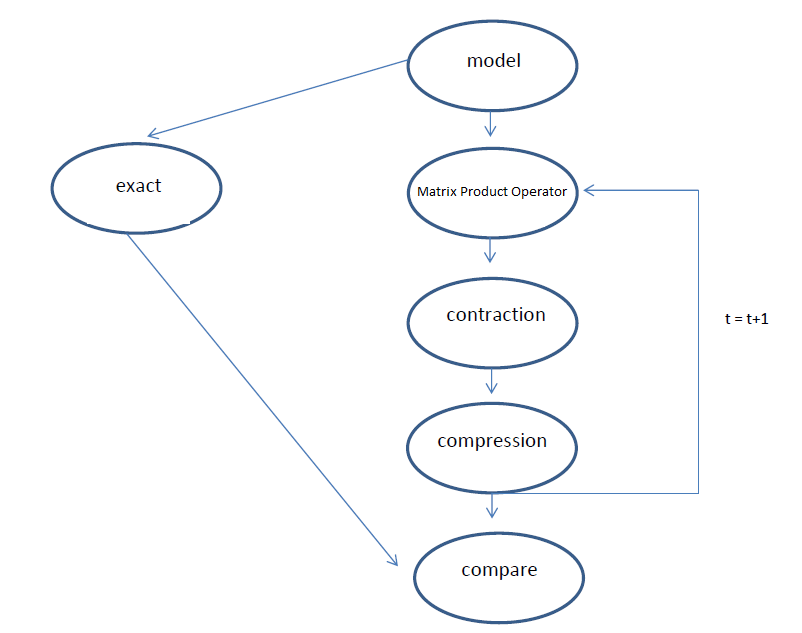
\includegraphics[width=\textwidth]{flow_chart.PNG}
\caption{The flow chart of our program.}
\label{fig:flow_chart}
\end{center}
\end{figure}

The implementation is summarized in Fig.~\ref{fig:flow_char}. The model will be implemented in two ways.

\subsubsection{Exact Solution}

An exact solution may be obtained for the proposed system. Because the dimension of state space grows exponentially, implementing such a solution becomes too computationally costly when dealing with a few dozen spins and/or chain sites. Nonetheless, an exact solution bounded by reasonably-sized state spaces will be needed to corroborate results obtained through the MPS algorithm.
To generate an exact solution for reasonably-sized state-spaces, a class Exact will be implemented. The class will contain two functions.  A function Interpreter will read data contained in an instance of the class Model, including the length of the chain and local dimensions for each chain site. This data will be used to construct a transitional matrix, to be implemented as a sparse matrix, which will be used for simulating the current state of the system. The interpreter will then call on the Step function to solve for the state by stepping in discrete time.
Additionally, a Monte Carlo simulation can be used to solve this problem. If time permits, a Monte Carlo simulation of the system will be implemented to serve as an addition comparator to the MPS algorithm.


\subsubsection{MPS class}
Parallel to the class \texttt{Exact}, we construct a class named \texttt{MPS} to store the MPS representation of the current state, to hold the MPO representation of the dynamic of the system and to comprise several functions which are necessary in updating the current state. The \texttt{MPS} class will include the following:

\vspace{3mm}
\noindent\textbf{Member data} We will have the current state in a variable named \texttt{MPState} which is a 3-d array storing $M^{\sigma_i}_{a_{i-1},a_i}$. The operator $O^{\sigma_i, \sigma'_i}_{n_{i-1}, n_i}$ will be stored in a variable named \texttt{MPO} which is a 4-d array. In addition, we will store the time of the system in the variable \texttt{T}.

\vspace{3mm}
\noindent\textbf{Constructor} The constructor will take a model of type \texttt{Model} and a initial state as argument and initilize the members \texttt{MPState}, \texttt{MPO} and \texttt{T}. Since we only focused on certain well-studied models and start the system from a given state, the form of \texttt{MPState} and \texttt{MPO} will be easy.

\vspace{3mm}
\noindent\textbf{Methods} As is shown in the flow chart, to update the state from time $t$ to $t+1$, one must first apply the MPO to the MPS and then do the compression. The reason why the compression step is necessary is that after applying MPO to MPS, the resulting MPS will have a greater degree of freedom. The compression step consists of projecting the resulting MPS (which is of higher dimension) back to the initial space (of a lower dimension). We shall write the routine \texttt{Step} responsible for applying MPO and updating the current state \texttt{MPState}. This routine will call \texttt{Compression} to make sure that the new state has the desired degree of freedom.

Both \texttt{Step} and \texttt{Compression} will involve some basic operations of multiplication of arrays and summing over a certain number of indices (something like matrix multiplication). We shall implement these basic operations first, so \texttt{Step} and \texttt{Compression} can call these routines.

Note that if we would like to calculate the expectation of a physical quatity, or the marginal probability of a physical states, we have to do the "overlapping" operation of two MPS. This again involves a number of basic operations defined in the class \texttt{MPS}. So the members in the class \texttt{Measurement} which handles the evaluation of expectations and probabilities, should be able to call the routines in the class \texttt{MPS}.
\end{document}
